\documentclass[10pt,a4paper]{article}
\usepackage[utf8]{inputenc}
\usepackage[magyar]{babel}
\usepackage[T1]{fontenc}
\usepackage{amsmath}
\usepackage{amsfonts}
\usepackage{amssymb}
\usepackage{makeidx}
\usepackage{graphicx}
\usepackage[pdfusetitle]{hyperref}
\usepackage{titling}

\hypersetup{
    colorlinks,
    citecolor=black,
    filecolor=black,
    linkcolor=black,
    urlcolor=black
}

\date{\today}
\author{Petrányi Bálint}
\title{%
	\textbf{Analízis 2.} \\
	\textbf{Programtervező informatikus A. szakirány} \\
	\medskip
	Bizonyítások\\
	\large 2022-2023. tanév 1. félév
}

\newcommand{\R}{\mathbb{R}}
\newcommand{\D}{\mathcal{D}}
\newcommand{\fR}{f\in\R\rightarrow\R}
\newcommand{\pf}{+\infty}
\newcommand{\nf}{-\infty}
\newcommand{\f}[1][x]{f(#1)}
\newcommand{\g}[1][x]{g(#1)}
\newcommand{\fg}{\Big(\frac{f}{g}\Big)}

\begin{document}
\maketitle
\tableofcontents
\newpage
\section{A differenciálhatóság átfogalmazása}
\textbf{Tétel:} \\ 
Legyen $f \in \mathbb{R} \rightarrow \mathbb{R}, a \in \text{int } \mathcal{D}_f$. Ekkor
\[
\begin{split}
f \in & \; D\{a\} \\
& \Updownarrow \\
\exists A \in \mathbb{R}, \; \text{és} \; \epsilon : \mathcal{D}_f \rightarrow \mathbb{R}, \lim_a{\epsilon} = 0 \quad \text{úgy, hogy } & \; f(x)- f(a) = A(x-a)+\epsilon (x)(x-a)
\end{split}
\]
\textbf{Bizonyítás:}
\[
\Longrightarrow f \in D\{a\} \; \text{esetén legyen} \; A:=f'(a), \; \text{és} \epsilon (x) := \frac{f(x)-f(a)}{x-a} -f'(a).
\]
Ezzel a választással egyrészt
\[
A(x-a) + \epsilon (x)(x-a) =f'(a)(x-a)+\Big(\frac{f(x)-f(a)}{x-a}-f'(a)\Big)(x-a) =f(x)-f(a),
\]
másrészt a differenciálhatóság miatt
\[
\lim\limits_{x\rightarrow a} \epsilon (x) = \lim\limits_{x\rightarrow a} \frac{f(x)-f(a)}{x-a}-f'(a)=0.
\]
$\Longleftarrow$ Ha az $A$ szám és az $\epsilon$ függvény teljesítik az állítást feltételeit, akkor 
\[
\frac{f(x)-f(a)}{x-a} = A + \epsilon (x), és \lim\limits_{x-a} \frac{f(x)-f(a)}{x-a} = A = f'(a) \in \mathbb{R}
\]
\newpage
\section{A szorzat függvény deriválása}
\textbf{Tétel:}
\[
f\in D\{a\} \Longrightarrow    f\cdot g \in D\{a\},  \text{és}  (f\cdot g)'(a) =f'(a)g(a)+ f(a)g'(a)
\]
\textbf{Bizonyítás:}
\begin{align*}
\frac{(fg)(x)-(fg)(a)}{x-a} &= \frac{f(x)\cdot g(x)-f(a)\cdot g(a)}{x-a}\\
 &= \frac{\f\cdot\g-\f[a]\cdot\g-\f[a]\cdot\g[a]+\f[a]\cdot\g}{x-a} \\
 &= \frac{\f-\f[a]}{x-a}\cdot\g + \f[a] \cdot \frac{\g-\g[a]}{x-a} \quad (x\in\D_{f\cdot g} \setminus \{a\})
\end{align*}
következés képen 
\[
\triangle_a f \cdot\g = \g \cdot \triangle_a\f\cdot + \f[a] \cdot \triangle_a\g \quad (x\in\D_{f\cdot g} \setminus \{a\})
\]
Mivel $g\in D \{a\}$ , ezét $g\in C\{a\}$ és így $\lim_a g = \g[a]$
\\ Ezek alapján:
\begin{align*}
(f\cdot g)'(a) & = \lim\limits_a \triangle_a (f\cdot g) = \lim\limits_a (g\cdot \triangle_a f ) + \lim\limits_a (\f[a]\cdot\triangle_a g ) \\
& =\g[a]\cdot f'(a) + \f[a]\cdot g'(a)
\end{align*}
\newpage
\section{A hányados függvény deriváltja}
\textbf{Tétel:}
\[
f\in D\{a\} \text{ és }  g(a)\neq 0 \Longrightarrow  \frac{f}{g} \in D\{a\},  \text{és}  \Big(\frac{f}{g} \Big)' (a) = \frac{f'(a)g(a)-f(a)g'(a)}{g^2(a)}
\]
\textbf{Bizonyítás:} \\
kifejezzük a hányadosfüggvényt különbségi hányados függvényt a számláló és a nevező különbségi hányados függvényével 
\begin{align*}
\triangle_a\fg (x) &= \frac{\fg (x)-\fg (a)}{x-a} = \frac{\frac{\f}{\g}-\frac{\f[a]}{\g[a]}}{x-a}  \\
&=\frac{1}{\g[a]\g} \cdot \frac{\f\cdot\g[a] - \f[a]\g}{x-a} \\ 
&=\frac{1}{\g[a]\g} \Big(\frac{\f -\f[a]}{x-a} \cdot\g[a] -\f[a]\cdot\frac{\g -\g[a]}{x-a} \Big) \\
&=\frac{1}{\g[a]\g} (\g[a]\cdot\triangle_a \f -\f[a]\cdot\triangle_a \g )
\end{align*}
Innen mindkét oldal $a$-beli határértékét véve kapjuk a bizonyítandó 
\[
\fg '(a) = \frac{f'(a)\cdot\g[a] - \f[a]\cdot g'(a)}{g^2 (a)}
\]
összefüggést
\newpage
\section{A lokális szélsőértékre vonatkozó elsőrendű szükséges feltétel}
\textbf{Tétel:} \\
Tegyük fel, hogy az $f:\R\rightarrow\R$ függvénynek az $a\in\D_f$ pontban lokális szélsőértéke van és $f\in D\{a\}$ \\
Ekkor:
\[
f'(a)=0
\]
\textbf{Bizonyítás:} \\
Tegyük fel, hogy $f$-nek $a$-ban lokális maximuma van. Ekkor $\exists r>0$, hogy 
\[
\forall x \in (a-r,a+r) \text{esetén} \f \leq f(a), \text{azaz} \f - f(a) \leq 0.
\]  
Tekintsük az $f$ függvény $a$-hoz tartozó különbségi hányados-függvényét
\[
\frac{\f -f(a)}{x-a} \quad (x\in \D_f \setminus \{a\})
\]
Ha $a<x<a+r$, akkor $x-a>0$ és $\f- f(a)\leq 0$ miatt
\[
\frac{\f -f(a)}{x-a} \leq 0 \Longrightarrow \lim\limits_{x\rightarrow a+0} \frac{\f -f(a)}{x-a} = f'_+ (a) \leq 0 
\]
Ha viszont $a-r<x<a$ akkor $x-a<0$ és $\f - f(a) \leq 0$ miatt
\[
\frac{\f -f(a)}{x-a} \geq 0 \longrightarrow \lim_{x\rightarrow a-0} \frac{\f -f(a)}{x-a} = f'_- (a) \geq 0 
\]
Mivel $f\in D\{a\}$ ezért
\[
\underbrace{f'_- (a)}_{\geq 0}  = \underbrace{f'_+ (a)}_{\leq 0}  = f' a = 0  
\]
A bizonyítás hasonló akkor is, ha $f$-nek $a$-ban lokális minimuma van.
\newpage
\section{A Rolle-féle középértéktétel}
\textbf{Tétel:} \\
legyen $a,b \in \R$ és $a<b$ Tegyük fel hogy 
\begin{enumerate}
\item $f\in C[a,b]$
\item $f\in D(a,b)$
\item $f(a)=f(b)$
\end{enumerate}
Ekkor
\[
\exists \varepsilon \in (a,b) \quad \text{hogy} \quad f'(\varepsilon) = 0
\]
\textbf{Bizonyítás:} \\
$f\in C[a,b] \rightarrow$ (Weierstrass-tétel) $\exists \alpha, \beta \in [a,b]$ hogy
\[
f(\alpha) = \min_{[a,b]} f=:m \quad \text{és} \quad f(\beta)  = \max_{[a,b]} f=:M
\]
1.eset: $m=M$ Ekkor $f$ állandó, így $\forall \varepsilon \in (a,b)$ esetén $f'(\varepsilon) = 0$ \\
2.eset: $m\neq M$ Mivel $f(a)=f(b)$, ezért $\alpha$ és $\beta$ közül legalább az egyik (pl. $\alpha$) $(a,b)$-be esik \\
Ekkor $\varepsilon :=\alpha \in \text{int}\D_f = (a,b),$ és $f$-nek $\varepsilon$-ban lokális minimuma van.  \\
Mivel $f\in D\{\varepsilon\}$ ezért innen a szélsőértékékre vonatkozó elsőrendű szükséges feltételből következik, hogy $f'(\varepsilon) = 0$
\newpage
\section{A Lagrange-féle középértéktétel.}
\textbf{Tétel:}\\
Legyen $a,b\in\R$ és $a<b$. Tegyük fel hogy 
\begin{enumerate}
\item $f\in C [a,b]$
\item $f\in D(a,b)$
\end{enumerate}
Ekkor:
\[
\exists \varepsilon \in (a,b) \quad \text{hogy} \quad f'(\varepsilon) = \frac{f(b)-f(a)}{b-a}
\]
\textbf{Bizonyítás:}\\
az $(a,f(a))$ és a $(b,f(b))$ pontokon átmenő szelő egyenesének az egyenlete
\[
y = h_{a,b} (x) = f'(\varepsilon) = \frac{f(b)-f(a)}{b-a} (x-a) +f(a)
\]
igazoljuk hogy az 
\[
F(x) := \f - h_{a,b} (x) \quad (x\in [a,b])
\]
függvény kielégíti a Rolle-féle középérték feltételeit \\
Valóban, $f$ és $h_{a,b}$ mindketten folytonosak a $[a,b]$-n és deriválhatók $(a,b)$-n, ezért a különbségük, $F$ szintén rendelkezik ezekkel a tulajdonságokkal \\
Továbbá: 
\begin{align*}
F(a) &= f(a) - h_{a,b} (a) = f(a)-f(a) =0 \\
F(b) &= f(b)- h_{a,b} (b) = f(b) - (\frac{f(b)-f(a)}{b-a}(b-a)+f(a))=0
\end{align*}
tehát $F(a)=F(b)$ is teljesül a Rolle-tétel alapján tehát van olyan $\varepsilon \in (a,b)$ pont amelyre 
\[
F'(\varepsilon) = f'(\varepsilon) -h'_{a,b} (\varepsilon) = f'(\varepsilon) - \frac{f(b)-f(a)}{b-a} = 0
\] 
Következésképpen
\[
f'(\varepsilon) = \frac{f(b)-f(a)}{b-a}
\]
\newpage
\section{A Cauchy-féle középértéktétel.}
\textbf{Tétel:} \\
Legyen $a,b\in\R$ és $a<b$. Tegyük fel hogy 
\begin{enumerate}
\item $f,g\in C[a,b]$
\item $f,g\in D(a,b)$
\item $g'(x)\neq 0 (x\in (a,b))$
\end{enumerate}
Ekkor:
\[
\exists \varepsilon \in (a,b), \quad \text{hogy} \quad \frac{f'(\varepsilon)}{g'(\varepsilon)} = \frac{f(b)-f(a)}{g(b)-g(a)}
\]
\textbf{Bizonyítás:}\\
A 3. feltételből a Rolle-tétel alapján következik, hogy $g(a)\neq g(b)$ vagyis az állítás
jobb oldalának a nevezője nem $0$ \\
Valóban $g(a) = g(b)$-ből az következne, hogy $g$ deriváltja nulla az $(a,b)$ intervallum
legalább egy pontjában, amit kizártunk. \\
Legyen
\[
F(x):=\f -f(a) -\frac{f(b)-f(a)}{g(b)-g(a)}(g(x)-g(a)) \quad (x\in [a,b])
\]
Az $F$ függvény kielégíti a Rolle-tétel félteleit: folytonos $[a,b]$-n Deriválható $(a,b)$-n és $F(a)=F(b)=0$ \\
Következésképpen létezik olyan $\varepsilon \in (a,b)$ amelyre $F'(\varepsilon)=0$ azaz
\[
0=F'(\varepsilon) = f'(\varepsilon)  -\frac{f(b)-f(a)}{g(b)-g(a)} g'(\varepsilon)
\]
Mivel a feltételeink szerint $g'(\varepsilon)\neq 0$  ezért átrendezéssel azt kapjuk, hogy
\[
\frac{f'(\varepsilon)}{g'(\varepsilon)} = \frac{f(b)-f(a)}{g(b)-g(a)}
\]
\newpage 
\section{Nyílt intervallumon értelmezett deriválható függvények esetében a monotonitás és a derivált kapcsolata}
\textbf{Tétel:} \\
Legyen $I \subset \R $ nyílt intervallum. Tegyük fel hogy $f : I \rightarrow \R, \; f\in D(I)$\\ Ekkor:
\[
f\nearrow \quad \Longleftrightarrow \quad f'\geq 0.
\] 
\textbf{Bizonyítás:} \\
$\Longrightarrow$ Legyen $x\in I$ Ekkor tetszőleges
\begin{enumerate}
\item \[y\in I \; , y>x \quad \text{esetén} \quad f(y)\geq f(x), \quad \text{tehát} \quad \triangle_x f(y) = \frac{f(y)-f(x)}{y-x} \geq 0  \]
\item \[y\in I \; , y>x \quad \text{esetén} \quad f(y)\leq f(x), \quad \text{tehát} \quad \triangle_x f(y) = \frac{f(y)-f(x)}{y-x} \leq 0  \]
\end{enumerate}
következésképpen
\[
\triangle_x f(y)\geq 0 \quad (y\in I) \Longrightarrow f'(x) = \lim\limits_{y\rightarrow x} \triangle_x f(y) \geq 0
\]
$\Longleftarrow$ Indirekt tegyük fel, hogy $f'$ nem monoton növekedő 
Ekkor $\exists x,y \in , x<y$ amelyre $f(y)<f(x)$
A Lagrange-féle középérték-tétel feltételei teljesülnek az $[x,y]\subset I$ intervallumon. \\
Következésképen $\exists \varepsilon \in (x,y)$, hogy 
\[
f'(\varepsilon) = \frac{f(y)-f(x)}{y-x} < 0 \text{Ellentmondás!}
\]
\newpage
\section{A lokális szélsőértékre vonatkozó elsőrendű elégséges feltétel}
\textbf{Tétel:} \\
Legyen $\fR$, és a $a\in \text{int }\D_f$.\\
Tegyük fel hogy $\exists \delta >0$, amelyre $f\in D((a-\delta ,a+\delta )) $ és $f'$ előjelet vált $a$-ban \\
Ekkor $f$-nek szigorú lokális szélsőértéke van az $a$-ban \\
($+,-$) jelváltás esetén maximum és($-,+$) jelváltás esetén minimum \\ \\
\textbf{Bizonyítás}:\\
Elég a $(+,-)$ jelváltás esetén bizonyítani.
feltételből következik, hogy $\exists \epsilon >0$, hogy
\begin{align*}
f'(x)&>0 (a-\epsilon,a) \text{ és } f\in C\{a\} \text{ és igy  } f_{\big\lvert (a-\epsilon,a)\uparrow} \\
f'(x)&<0 (a,a+\epsilon), \text{ és } f\in C\{a\} \text{ és igy } f_{\big\lvert (a,a+\epsilon)\downarrow} \\
\end{align*}
Következésképpen $f(a)>\f \; \forall x \in (a-\epsilon,a+\epsilon) \setminus \{a\}$
\newpage
\section{A konvexitás jellemzése a deriváltfüggvénnyel.}
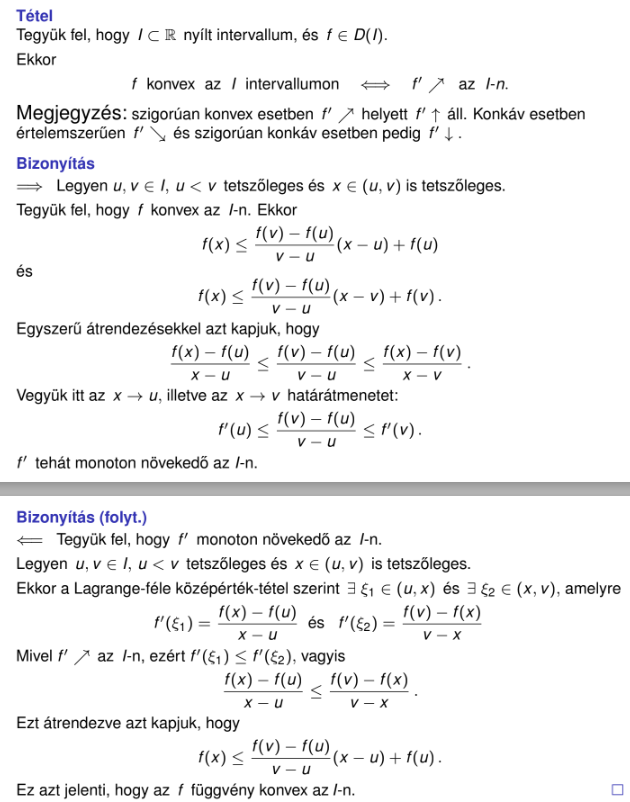
\includegraphics[scale=1]{10.PNG}
\newpage
\section{A véges pontbeli $\frac{0}{0}$ határérték esetre vonatkozo L'Hospital-szabály}
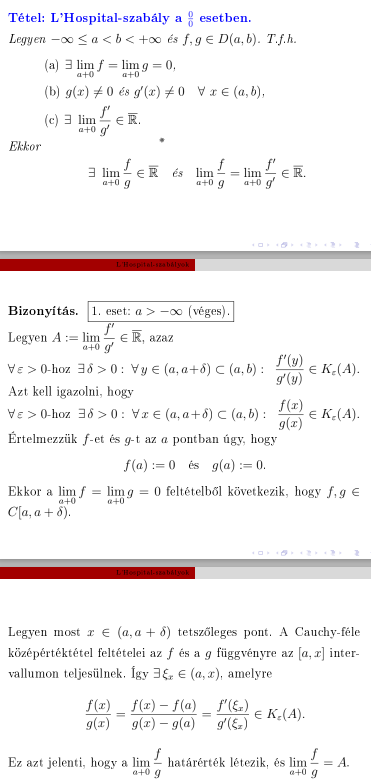
\includegraphics[scale=1]{11.PNG}
\newpage
\section{A Taylor-formula a Lagrange-féle maradéktaggal}
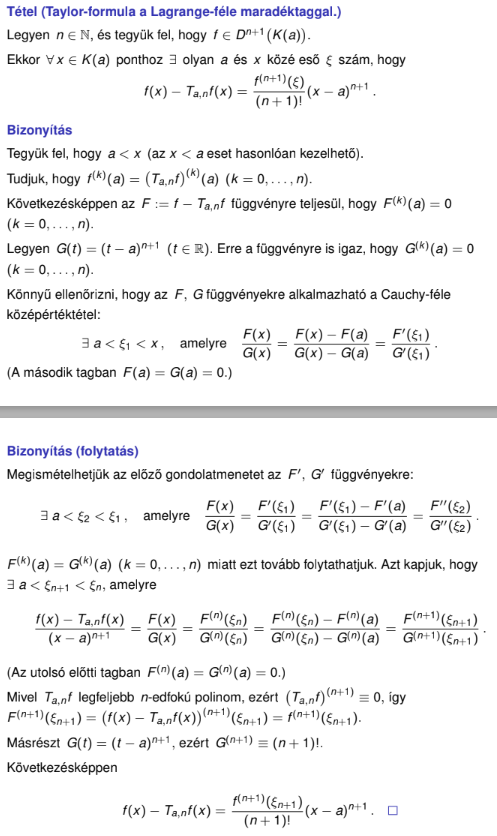
\includegraphics[scale=1]{12.PNG}
\end{document}